\chapter{Local Fourier Spectral Filters}
%We propose the use of Local Fourier-Spectral (LFS) filters, developed originally for 1-D and 2-D tensor-product elements by Asthana and López-Morales [cite], as a parameter-free approach to stabilize high-order solutions. The LFS filters stabilize the solution, when needed, under all potential modes of failure. Their formulation adapts easily to Finite-Element-based spatial discretizations: the filter has a compact stencil, is not more expensive than a solution evaluation, and is discretization-agnostic. We present solutions to turbulent, transonic, and supersonic flows using the Flux Reconstruction approach, a high-order scheme heavily studied in the Aerospace Computing Laboratory. All solutions are obtained in coarse, unstructured grids using a medium-cost multi-GPU-powered workstation.
%
%\subsection{Introduction}
%Mention that author was seeking filters that could be posed as a matrix-vector multiplication with a local stencil. Inspiration came from paper by Lodato.
%
%\subsection{Non-linear stabilization of high-order Flux Reconstruction schemes}
%Present summary of paper by Asthana et al. and key results.
%
%\subsection{1-D and 2-D tensor product element filtering approach}
%Describe original approach by Asthana et al. to filtering: basis functions outside element of interest are defined as constants in 1-D, and extruded curves and constants in 2-D.
%
%\subsection{Extension to arbitrary elements}
%Describe how filtering matrix is composed of two submatrices: square matrix that modifies the spectrum (energetic content) of the solution, and rectangular matrix that ensures the filter is Essentially Local Extremum Diminishing.
%
%The formulation of this type of filter is agnostic to the type of element and basis functions used, and provides a framework to design new LFS.
%
%\subsection{Simulations}
%\subsubsection{1D}
%\subsubsection{2D}
%\subsubsection{3D}

% !TEX root = ./thesis.tex

\section{Introduction}

During the last decade, the \gls{acl} of the Department of Aeronautics and Astronautics at Stanford University has developed a series of high-order numerical schemes and computational tools that have demonstrated the viability of this technique. In this chapter, the code named \gls{hf}, developed in the \gls{acl} and built on top of SD++ (Castonguay et al.\cite{castonguay2011}), is described in detail with a particular emphasis on robustness in a range of applications and \gls{vv}. \gls{hf} takes advantage of the synergies between applied mathematics, aerospace engineering, and computer science in order to achieve the ultimate goal of developing an advanced high-fidelity simulation environment.

In addition to the original characteristics of the SD++ code, \gls{hf} includes some important physical models and computational methods such as: \gls{les} using explicit filters and advanced \gls{sgs} models, high-order stabilization techniques, shock detection and capturing for compressible flow calculations, and local time stepping.

During the development of this software, several key decisions have been taken to guarantee a flexible and lasting infrastructure for industrial Computational Fluid Dynamics simulations:
\begin{itemize}
\item The selection of the \gls{esfr} scheme on unstructured grids\cite{vincent2011new}. The flexibility of this method has been critical to guarantee a correct solution independently of the particular physical characteristics of the problem.
\item High performance, materialized in a multi-\gls{gpu} implementation that takes advantage of the ease of parallelization afforded by discontinuous solution representation. Furthermore, \gls{hf} aims to guarantee compatibility with future vector machines and revolutionary hardware technologies.
\item Code portability by using ANSI C++ and relying on widely-available, and well-supported mathematical libraries like Blas, LAPACK, CuBLAS, and ParMetis.
\item Object oriented structure to boost the re-usability and encapsulation of the code. This abstraction enables modifications without incorrectly affecting other portions of the code. Although some level of performance is traded for re-usability and encapsulation, the loss in performance is minor.
\end{itemize}

As the mathematical basis and computational implementation of \gls{hf} have been described in previous work~\cite{castonguay2011}, the goal of this chapter is to illustrate the level of robustness of \gls{hf} for interesting problems. This will be accomplished via a \gls{vv} study, which is fundamental for increasing the credibility of this technology in a competitive industrial framework.

In particular, to ensure that the implementation of the aforementioned features in \gls{hf} is correct, the following verification tests are shown: checks of spatial and temporal order of accuracy using the \gls{mms} in 2D and 3D for viscous and inviscid flows and characterization of stable time-step limits. After the Verification, a detailed Validation of the code is presented to illustrate that the solutions provided by \gls{hf} are an accurate representation of the real world. Simulations of complex flows are validated against experimental or \gls{dns} results for the following cases: laminar flat-plane, flow around a circular cylinder, SD7003 wing-section and airfoil at 4$\degr$ angle of attack, the Taylor-Green Vortex, and \gls{les} of a square cylinder.

The organization of this chapter is as follows. Section~\ref{sec:govEq} provides a description of the governing equations. Section~\ref{sec:numerics} describes the mathematical and numerical algorithms implemented in the code. Section~\ref{sec:verification} focuses on the \gls{vv} of \gls{hf}, and the conclusions are summarized in Section~\ref{sec:conclusion_hf}. It is important to highlight that the contents of this chapter mirror the \gls{aiaa} paper\cite{lopez2014verification} created jointly with members of the \gls{acl} and Francisco Palacios.

\vspace{.20in}

\section{Flux Reconstruction Method}
\label{sec:frmethod}
What follows is a brief overview of the \gls{fr} framework with an emphasis on how the \gls{lfs} filtering technique can be seamlessly implemented. We start the discussion with the solution of the advection equation in one dimension using the \gls{fr} approach to illustrate the method. We then proceed to briefly explain how conservation equations can be solved in multiple dimensions. The \gls{ns} equations are a set of coupled conservation equations in multiple dimensions, so the extension of the \gls{fr} methodology to them is straightforward. The detailed description of the algorithm used in \gls{hf} is given by Castonguay et al.~\cite{castonguay2011}.

\subsection{Solution of the Advection Equation in One Dimension using the FR Approach}

Consider the one-dimensional conservation law
\begin{equation}
\label{eq:cons}
\frac{\partial u}{\partial t} + \frac{\partial f}{\partial x} = 0
\end{equation}

in domain $\Omega$, where $x$ is the spatial coordinate, $t$ is time, $u$ --the \emph{solution}-- is a scalar function of $x$ and $t$, and $f$ --the \emph{flux}-- is a scalar function of $u$. Note that by letting $f = f(u,\frac{\partial u}{\partial x})$, Equation~\eqref{eq:cons} becomes a model of the Navier-Stokes equations.

Let us partition the domain $\Omega = [x_1,x_{N+1})$ into $N$ non-overlapping elements with 
interfaces at $x_1<x_2<...<x_{N+1}$. Then,
\begin{equation}
\Omega = \bigcup^N_{n=1} \Omega_n
\end{equation}
and $\Omega_n = [x_n,x_{n+1})$ for $n = 1,...,N$. To simplify the implementation, let us map each of the physical elements $\Omega_n$ to a standard element $\Omega_s=[-1,1)$ with the function $\Theta_n(\xi)$, where
\begin{equation}
x = \Theta_n(\xi) = \l( \frac{1-\xi}{2} \r) x_n + \l(\frac{1+\xi}{2}\r) x_{n+1} 
\end{equation}

With this mapping, the evolution of $u$ within each $\Omega_n$ can be determined with the following 
transformed conservation equation
\begin{equation}
\frac{\partial \hat{u}}{\partial t} + \frac{1}{J_n}\frac{\partial \hat{f}}{\partial \xi} = 0,
\end{equation}
where
\begin{equation}
\hat{u} = u(\Theta_n(\xi),t) \text{ in } \Omega_n,
\end{equation}
\begin{equation}
\hat{f} = f(\Theta_n(\xi),t) \text{ in } \Omega_n,
\end{equation}
\begin{equation}
J_n = \frac{\partial x}{\partial \xi} \bigg|_{\Omega_n}.
\end{equation}

Now, we introduce polynomials of degree $p$, $\hat{u}^\delta$ and $\hat{f}^\delta$, to approximate the exact values $\hat{u},\hat{f}$, respectively. We can write these polynomials as
\begin{equation}
\hat{u}^\delta = \sum_{i=1}^{N_s} \hat{u}_i^\delta l_i(\xi),
\end{equation}
\begin{equation}
\hat{f}^\delta = \sum_{i=1}^{N_s} \hat{f}_i^\delta l_i(\xi),
\end{equation}
where $N_s$ is the number of solution points, $\hat{u}_i^\delta$ is the current value of the 
solution approximation function at the $i^\text{th}$ \emph{solution point} (or \emph{internal point}) in the reference element, 
$\hat{f}_i^\delta$ is the current value of the flux approximation function at the $i^\text{th}$ 
\emph{flux point} (or \emph{boundary point}) in the reference element, $l_i$ is the Lagrange polynomial equal to $1$ at the 
$i^\text{th}$ solution point and $0$ at the others, and $\delta$ denotes that the function is an 
approximation.

Note that the piecewise polynomials might not be continuous (or $C^0$) across the interfaces. In the 
Flux Reconstruction approach, the flux used in the time advancement of the solution is made $C^0$ 
by introducing flux correction functions.

This can be achieved by finding interface solution values at each element boundary and then correcting the 
solution. Let $\hat{f}_L^{\delta I}$ and $\hat{f}_R^{\delta I}$ be the interface flux values at left and right 
boundaries of some element, respectively. $\hat{f}_L^{\delta I}$ and $\hat{f}_R^{\delta I}$ can be found with a Riemann solver for \gls{dg} methods\cite{hesthaven2007nodal}. Then, select solution correction functions $h_L$ and 
$h_R$ such 
that
\begin{equation}\label{eq:condition}
h_L(-1) = 1 \;,\; h_L(1) = 0,
\end{equation}
\begin{equation}
h_R(-1) = 0 \;,\; h_R(1) = 1,
\end{equation}
and let
\begin{equation}
\hat{f}^C = \hat{f}^\delta + (\hat{f}^{\delta I}_L - \hat{f}^\delta_L) h_L + (\hat{f}^{\delta I}_R 
- \hat{f}^\delta_R) h_R,
\end{equation}
where superscript $C$ denotes the function is corrected, and $\hat{f}^\delta_L$, $\hat{f}^\delta_R$ 
represent the flux approximation evaluated at the left and right boundaries.

The solution can then be advanced at each solution point $i$ in element $n$. In semi-discrete form, this is
\begin{equation}\label{eq:semidiscrete}
\frac{d \hat{u}_i^\delta}{d t} = - \frac{1}{J_n}\frac{\partial \hat{f}^C}{\partial \xi}(\xi_i).
\end{equation}

The \gls{fr} scheme can be made provably stable for the linear advection-diffusion equation by selecting special types of correction functions~\cite{castonguay2013energy}. In general, these correction functions are polynomials of degree $p+1$ so both sides in Equation~\eqref{eq:semidiscrete} are quantities related to polynomials of order $p$ --for consistency~\cite{huynh2007flux}.

Vincent et al.~\cite{vincent2011new} have shown that in the case of the 1-dimensional, linear advection equation, the \gls{fr} approach can be proven to be stable for a specific family of correction functions parameterized by a scalar called $c$. In addition, they showed that by selecting specific values of $c$ it is possible to recover a particular nodal \gls{dg} and \gls{sd} methods plus a \gls{fr} scheme that was previously found to be stable by Huynh\cite{huynh2007flux}.

\subsection{Extension to Multiple Dimensions}

Extension of \gls{fr} to multiple dimensions requires formulating multi-dimensional interpolation functions and correction functions that satisfy boundary conditions equivalent to those in Equation~\eqref{eq:condition} for each type of element.

Interpolation bases for quadrilaterals and hexahedra can be obtained via tensor products of the 1-dimensional interpolation basis. In \gls{hf}, the solution in hexahedra is discretized in the following way
\begin{equation}
{\hat{u}}^\delta(\xi,\eta,\zeta) = \sum_{i=1}^{p+1} \sum_{j=1}^{p+1} \sum_{k=1}^{p+1}
{\hat{u}}^\delta_{i,j,k} l_i(\xi) l_j(\eta) l_k(\zeta),
\end{equation}
where $i$, $j$, $k$ index the solution points along the $\xi, \eta, \zeta$ directions, respectively. The flux is discretized similarly.

The interpolation basis for triangles and tetrahedra are described in detail by Hesthaven and Warburton~\cite{hesthaven2007nodal}. Figure \ref{fig:tri_points} shows a possible configuration of internal and boundary points. The extension of interpolation polynomials to prisms is obtained via tensor products of the 1-dimensional basis with the triangular basis~\cite{castonguay2011}. 

The most general polynomial discretization of a $k$-dimensional solution scalar field and flux vector field in an arbitrary reference element is
\begin{align}
\label{eqn:general_u}
\hat{u}^\delta({\pmb \xi}) &= \sum_{i=1}^{N_s} \hat{u}_i^\delta {\phi}_i({\pmb \xi}),\\
\hat{\bf f}^\delta({\pmb \xi}) &= \sum_{i=1}^{N_s} \hat{\bf f}_i^\delta {\phi}_i({\pmb \xi}),
\end{align}
where $N_s$ is the number of solution points in an element, ${\phi}_i({\pmb \xi})$ is a polynomial basis function associated with solution point $i$ constructed such that ${\phi}_i({\pmb \xi}_j) = \delta_{ij}$ and $i,j = 1,\dots,N_s$.

By letting $\vec{u} = <\hat{u}_1^\delta, \hat{u}_2^\delta,\dots,\hat{u}_{N_s}^\delta>^T $, $\vec{\bf f} = <\hat{\bf f}_1^\delta, \hat{\bf f}_2^\delta,\dots,\hat{\bf f}_{N_s}^\delta>^T $, and $\vec{\phi} = <\phi_1,\phi_2,\dots,\phi_{N_s}>^T$ the discretization can be written more concisely as
\begin{equation}
\begin{split}
\hat{u}^\delta({\pmb \xi}) &= \vec{u}^T \cdot \vec{\phi}({\pmb \xi}) =  \vec{\phi}({\pmb \xi})^T\cdot \vec{u},\\
\hat{\bf f}^\delta({\pmb \xi}) &= \vec{\bf f}^T \cdot \vec{\phi}({\pmb \xi}) = \vec{\phi}({\pmb \xi})^T \cdot \vec{\bf f}.
\end{split}
\end{equation}

Note that we are using the boldface and arrow notation to denote vectors. Boldface vectors have a number of entries equal to the number of dimensions of the problem domain. Arrow vectors are vectors of general dimensions.

In the general \gls{fr} approach, the boundary conditions for the correction functions in multiple dimensions can be formulated as
\begin{equation}\label{eq:genConstraint}
{\bf{h}}_i( {\pmb \xi}_j)\cdot {\bf{n}}_j = \delta_{ij},
\end{equation}
where ${\bf{h}}_i$ is the correction vector function associated with interface point $i$, ${\pmb \xi}_j$ is the location vector of the $j^\text{th}$ interface point, and ${\bf{n}}_j$ is the outward unit normal at interface point $j$. Interface (or boundary) points are located on the boundary of an element.

One of the challenges in the \gls{fr} approach is finding correction functions that not only satisfy Equation~\eqref{eq:genConstraint} but also guarantee stability in the linear advection-diffusion case. Correction functions that guarantee such stability exist for 1-dimensional segments\cite{vincent2011new}, triangles\cite{castonguay2012new,williams2013tri}, and tetrahedra\cite{williams2013tet}. FR schemes with these correction functions comprise the ESFR family of schemes.

The update step at solution point $i$ and element $n$ in the \gls{fr} approach for the multidimensional advection equation $\frac{\partial u}{\partial t} + \nabla \cdot \vec{f} = 0$ becomes
\begin{equation}
\label{eqn:discrete}
\begin{split}
\frac{d {u}^\delta_i}{d t} &= - \frac{1}{\text{det}(\tilde{J_n})} \nabla \cdot {\bf f}_i^C({\pmb \xi}_i) = - \frac{1}{\text{det}(\tilde{J_n})} \nabla \cdot \l({\bf f}_i^\delta({\pmb \xi}_i) + \sum^{N_f}_{j = 1} \l[\l( \hat{\bf f}^{\delta I}_j - \hat{\bf f}^b_j \r)\cdot {\bf n}_j \r]\vec{\bf h}_j ({\pmb \xi}_i) \r)\\
&=- \frac{1}{\text{det}(\tilde{J_n})} \l( \nabla \cdot {\bf f}_i^\delta({\pmb \xi}_i) + \sum^{N_f}_{j = 1} \l[\l( \hat{\bf f}^{\delta I}_j - \hat{\bf f}^b_j\r)\cdot {\bf n}_j \r]\nabla \cdot\vec{\bf h}_j ({\pmb \xi}_i)\r)\\
&=- \frac{1}{\text{det}(\tilde{J_n})} \l( \vec{\nabla \phi}({\pmb \xi}_i)^T  \cdot  \vec{\bf f} + \sum^{N_f}_{j = 1} \l[\l( \hat{\bf f}^{\delta I}_j - \hat{\bf f}^b_j\r)\cdot {\bf n}_j \r]\nabla \cdot\vec{\bf h}_j ({\pmb \xi}_i)\r),\\
\end{split}
\end{equation}
where $N_f$ is the number of interface points, $\tilde{J_n}$ is the Jacobian matrix, $\vec{\nabla \phi}({\pmb \xi}_i)$ is the vector of gradients of each $\phi_i$ function evaluated at ${\pmb \xi}_i$, $\vec{\bf f}^\delta$ is a vector of flux vectors, and $\hat{\bf f}^b_j$ is the flux vector at the $j^{\text{th}}$ interface point (obtained via extrapolation).

Note that it is possible to evaluate each of the terms in Equation \eqref{eqn:discrete} for all $i = 1,\dots,N_s$ with a series of matrix-vector multiplications.



\vspace{.20in}

\section{Local Fourier Spectral Filters}
\label{sec:lfsfilter}

\subsection{Desired Properties}
\label{sec:lfs_properties}
When designing the \gls{lfs} Filters presented in this paper, we considered the following properties as desirable:
\begin{enumerate}[1. ]
\item The filter should have spectral interpretation so there is control over the physical scales being smoothed
\item \label{item:local_stencil} The filtering operation must have a local stencil: only interior and boundary solution values can be used to filter the solution in the interior of the element
\item \label{item:filt_bc}The filter should preserve boundary conditions
\item \label{item:filt_bi}Filtering the solution at the interior points should be influenced by the solution values at the element's boundary
\item \label{item:influence}The influence of a boundary point on the internal point being filtered should be inversely proportional to the distance between them
\item To limit computational cost, the filter should be applied in the reference domain and involve matrix-vector multiplications exclusively

\item \label{item:generalizability}Filtering strategy should be generalizable to any type of element in unstructured grids

In the early stages of the filter design, we noted that Properties \ref{item:filt_bc} and \ref{item:filt_bi} could be overly stringent, so we re-phrased them as the following, more relaxed condition:

\item \label{item:coplanar}If solution values at the boundary lie on a hyperplane in the space of spatial coordinates and solution values, the filtering operation should bring the internal solution values closer to such plane. In other words, if the solution values at the boundaries can be determined from a linear function of their location, the filter should bring the internal solution values closer to satisfying such linear function.
\end{enumerate}



Condition \ref{item:coplanar} may not allow a filtered solution to satisfy the boundary conditions always. Nevertheless, in the limit of infinite mesh refinement the solutions at the boundary of every element will be coplanar, even in the presence of shocks in the \gls{ns}  equations. Hence, Condition \ref{item:coplanar} satisfies conditions \ref{item:filt_bc} and \ref{item:filt_bi} asimptotically. This re-formulation was inspired by the \gls{eled}  property of the \gls{jst}  scheme\cite{jameson1981numerical} for finite volume methods. Whether or not (some) \gls{lfs} filters satisfy \gls{eled}  properties shall be left for a future study.

%At this point it is important to note the main difference between the filters being proposed here and the commonly used modal filters\cite{kanevsky2006idempotent}. Modal filters are not influenced by the values of the solution at the boundary points. Therefore, if an element is experiencing aliasing, a modal filter will not necessarily ``nudge" the internal solution values towards continuity with its neighbors. In addition, in the limit of mesh refinement, modal filtering might not enforce an element's boundary conditions.

\subsection{Mechanics of \gls{lfs} Filters}

The core idea of the \gls{lfs} filtering technique is that the solution is filtered with a matrix whose entries depend on the element interface values, the basis functions of the solution, and a selected Fourier filtering kernel.

Suppose we wish to filter the scalar field $v$ inside an arbitrary element. This field could be density, momentum in a specific direction, or energy. We can represent $v$, as usual, as a weighted sum of basis functions.
\begin{equation}
\label{eqn:polyexp}
v(\bxi) = \sum^{N_s}_{i=1} v_i \phi_i(\bxi),
\end{equation}
where $v_i$ is the \ith weight, $\bxi$ is a vector of coordinates in a reference domain, and $\phi_i(\bxi)$ is the \ith basis function.

The key component of the \gls{lfs} technique is that the Fourier filtering operation over the element is approximated at each internal point $i$ with coordinates $\bxi_i$. Suppose we wish to use filtering kernel $G(\bxi)$ to filter $v(\bxi)$, then the filtered value at internal point $i$ becomes
\begin{equation}
\label{eqn:convolution}
\begin{split}
\bar{v}_j &= (G \ast v)(\bxi_j)\\
&= \int_{\mathbb{R}^d} G(\bxi_j - \bxi)v(\bxi)d\bxi\\
&= \int_{\mathbb{R}^d} G(\bxi_j - \bxi)\l(\sum^{N_s}_{i=1} v_i \phi_i(\bxi)\r)d\bxi\\
&= \sum^{N_s}_{i=1}v_i\int_{\mathbb{R}^d} G(\bxi_j - \bxi)  \phi_i(\bxi)d\bxi,\\
\end{split}
\end{equation}

where $\Omega$ is the entire problem domain, not just the element domain, $N_s$ is the number of solution points, and the overbar means the quantity is filtered. Filtering over the entire domain would be computationally expensive, but would certainly smoothen the solution field and can be done while maintaining the order of accuracy of the underlying numerical scheme\cite{mirzaee2012efficient,steffen2008investigation,walfisch2009one}. In order to use only a local (element-wise) stencil, it is possible to break the integration as follows
\begin{equation}
\label{eqn:brokenint}
\int_{\mathbb{R}^d} G(\bxi_j - \bxi)  \phi_i(\bxi)d\bxi = \int_{\Omega_n} G(\bxi_j - \bxi)  \phi_i(\bxi)d\bxi + \int_{\mathbb{R}^d \backslash \Omega_n} G(\bxi_j - \bxi)  \phi_i(\bxi)d\bxi,
\end{equation}
where $\Omega_n$ is the domain of element $n$ (where the $\phi_i$ values are known) and $\Omega \backslash \Omega_n$ is the complement of $\Omega_n$ in $\Omega$. As $G$ and $\phi_i$ are defined in $\Omega_n$, it is possible to calculate the first integral in Equation \eqref{eqn:brokenint} analytically or via an adaptive quadrature algorithm like \texttt{quanc8}~\cite{forsythe1977computer}.

A design choice arises in defining $\phi_i$ in the domain $\Omega \backslash \Omega_n$. Asthana et al.~\cite{asthana2014} initially decided to let $\phi_i$ equal a constant in 1D elements, and a combination of constant and polynomial in quadrilaterals. Non-tensor-product elements became problematic for this kind of formulation. This paper presents a more generic filter design method based on the desired properties in Section \ref{sec:lfs_properties}.

Let us describe the mechanics of the two components of the integral in Equation \eqref{eqn:brokenint} in a subsection each. We can call the filter associated with the term $\int_{\Omega_n} G(\bxi_j - \bxi)  \phi_i(\bxi)d\bxi$ ``Internal Filtering Component" and the filter associated with the term $\int_{\mathbb{R}^d \backslash \Omega_n} G(\bxi_j - \bxi)  \phi_i(\bxi)d\bxi$ ``Boundary Filtering Component".

The filtering operation being sought follows this format
\begin{equation}
\label{eqn:filter_form}
\vec{\bar{v}} = \alpha\mat{T}\vec{v} + (1-\alpha)\mat{B}\vec{v^*},
\end{equation}
where $\mat{T}$ is the internal filtering component, as it acts on the solution at internal points $\vec{v}$, and $\mat{B}$ is the boundary filtering component, as it acts on the solution at boundary points $\vec{v^*}$, and $\alpha$ is a scalar between $0$ and $1$ that determines the relative influence the internal and boundary components have on the internal solution values.

\subsection{Internal Filtering Component}
There are two steps to the creation of the internal filtering component $\mat{T}$. First we create the filtering matrix with the spectral interpretation, and then we normalize it so if the quantity being filtered is a constant, the filter preserves the constant.
\subsubsection{Matrix formation}
It can be seen from the last line in Equation \eqref{eqn:convolution} that finding the vector of solution values filtered with the internal component can be posed as a matrix-vector multiplication:
\begin{equation*}
\label{eq:internal_matrix}
\begin{bmatrix}
\bar{v}_1 \\
\bar{v}_2 \\
\vdots\\
\bar{v}_{N_s} \\
\end{bmatrix} = 
\begin{bmatrix}
\int_{\Omega_n} G(\bxi_1 - \bxi)  \phi_1(\bxi)d\bxi &
\int_{\Omega_n} G(\bxi_1 - \bxi)  \phi_2(\bxi)d\bxi &
\cdots &
\int_{\Omega_n} G(\bxi_1 - \bxi)  \phi_{N_s}(\bxi)d\bxi\\
\int_{\Omega_n} G(\bxi_2 - \bxi)  \phi_1(\bxi)d\bxi &
\int_{\Omega_n} G(\bxi_2 - \bxi)  \phi_2(\bxi)d\bxi &
\cdots &
\int_{\Omega_n} G(\bxi_2 - \bxi)  \phi_{N_s}(\bxi)d\bxi\\
\vdots & \vdots & \ddots & \vdots\\
\int_{\Omega_n} G(\bxi_{N_s} - \bxi)  \phi_1(\bxi)d\bxi &
\int_{\Omega_n} G(\bxi_{N_s} - \bxi)  \phi_2(\bxi)d\bxi &
\cdots &
\int_{\Omega_n} G(\bxi_{N_s} - \bxi)  \phi_{N_s}(\bxi)d\bxi
\end{bmatrix}
\begin{bmatrix}
v_1 \\
v_2 \\
\vdots\\
v_{N_s} \\
\end{bmatrix}.
\end{equation*}

More compactly,
\begin{equation}
\label{eqn:filtmat}
\vec{\bar{v}} = \mat{F}\vec{v}
\end{equation}
we use over-arrow to denote column vectors.
Interesting choices for $G(\bxi)$ depend on a desired wavenumber threshold $h$:

\begin{enumerate}[I.]
\item Gaussian function:
$$
G(\bxi) = h \exp{(h||\bxi||)},
$$
where $||\bxi||$ is a measure of the length of $\bxi$.
\item \label{item:multi_ind_func}Multidimensional indicator function:
$$
G(\bxi) = h\mathrm{I}_{[0,1]}(h||\bxi||),
$$
where $\mathrm{I}_{[0,1]}(x) = 1 \text{ if } 0\le x\le 1$, and $0$ otherwise.
\item \label{item:sharp_spectral}Multidimensional sharp-spectral function:
$$
G(\bxi) = h||\bxi||^{-n/2}
J_{n/2}(h||\bxi||),
$$
where $J_\alpha$ is a Bessel function of the first kind and $n$ is the number of dimensions of $\bxi$.
\end{enumerate}

In these functions, the larger the value of $h$, the thinner the filter is in physical space, so the fewer wavenumbers it dampens. Note that as $h \rightarrow \infty$, $\mat{F}_{ij}  \rightarrow \phi_j(\bxi_i)$, so $\vec{\bar{v}} \rightarrow \vec{{v}}$. The integrals in Equation \eqref{eq:internal_matrix} can be evaluated to arbitrary accuracy with \texttt{quanc8}~\cite{forsythe1977computer} in a pre-processing stage.

\subsubsection{Enforcing Conservation of a Constant Quantity}
The requirement to preserve a constant can be posed in an equation as
\begin{align}
\bar{v}_i = \sum^{N_s}_{j = 1} \mat{F}_{ij} v_{\text{const}} = v_{\text{const}},
\end{align}
where $v_{\text{const}}$ is a constant scalar. As a result, each row of $\mat{F}$ must satisfy
\begin{align}
\sum^{N_s}_{j = 1} \mat{F}_{ij} = 1,
\end{align}
where $i = 1,\dots,N_s$.
This constraint can be enforced by dividing each row of $\mat{F}$ with the total sum of the row. More explicitly,
\begin{align}
{\mat{T}}_{ij} = \frac{\mat{F}_{ij}}{\sum^{N_s}_{k = 1} \mat{F}_{ik}},
\end{align}
where the normalized matrix ${\mat{T}}$ is the internal filtering component in Equation \eqref{eqn:filter_form}.

\subsubsection{Integration Domain}

The normalization of the matrix introduces a bias. As the integration is being performed in some reference domain $\Omega_n$, the integral $\int_{\Omega_n} G(\bxi_i - \bxi)  \phi_j(\bxi)d\bxi$ will tend to have a greater value when $\bxi_i$ is well inside the reference element. This is more evident when using the multidimensional indicator function (shown in \ref{item:multi_ind_func}) as the filtering kernel.

To ameliorate this bias, we have selected to perform the integration in a reference domain that is symmetric. With this precaution all integrals related to points close to a domain edge have a similar magnitude, and thus the filtering operation does not favor points close to some arbitrary edge over the others.

Figure \ref{fig:domain_example} illustrates the potential introduction of bias in triangular elements that use a right triangle as a reference element.

\begin{figure*}

\subfloat[Equilateral triangle domain\label{fig:equi_tri_domain}]{%
      \includegraphics[width=0.45\textwidth]{\lfsdir/figs/equi_tri.pdf}
    }
    \hfill
    \subfloat[Right triangle domain\label{fig:right_tri_domain}]{%
          \includegraphics[width=0.45\textwidth]{\lfsdir/figs/right_tri.pdf}
        }
\caption{Using the same filter width in two different domains introduces different bias. The small, solid circles represent the location of solution points. The large circles represent the filter width acting on two specific internal points in two different domains. Integration is being performed in the area encompassed by the solid, straight lines.}
\label{fig:domain_example}

\end{figure*}

In practice, the basis functions $\phi_j(\bxi)$ may be defined in non-symmetrical elements. To simplify the evaluation of the integral, the definition of the norm in the filtering kernel $G(\bxi)$ can be modified so the curve drawn by $||\bxi -\bxi_0|| = 1$ in the non-symmetric reference element would map to a circle in a symmetric reference element.

In the case of a triangle, the basis functions are defined in a right triangle with vertices $[-1,-1], [1,-1],[-1,1]$.

By defining the norm in this right triangle as follows
\begin{equation}
\label{eqn:rect_norm}
||\bxi||^2_{rt} = \bxi_1^2 + \bxi_2^2 + \bxi_1\bxi_2,
\end{equation}
$||\bxi -\bxi_0||_{rt} = 1$ maps to a circle in the equilateral triangle with vertices $[-1,-1],[1,-1],[0,\sqrt{3}-1]$. Figure \ref{fig:mapping} sketches this mapping. $||\cdot||_{rt}$ is the norm defined in the right triangle.


\begin{figure}\centering
\includegraphics[width = 0.75\textwidth]{\lfsdir/figs/mapping.pdf}
\caption{Sketch of ellipsis $||\bxi -\bxi_0||_{rt} = 1$ defined in the right triangle domain maps to a circle in the equilateral triangle domain}
\label{fig:mapping}
\end{figure}

\subsection{Boundary Filtering Component}

Formulating the influence of boundary solution values on internal solution values as a matrix is not so straightforward. The approach being suggested here is based on some reasonable desired properties, but some choices are arbitrary. 

The creation of this matrix proceeds as follows: place the boundary points and the internal points in a symmetric domain, select an ``influence" function with as many unknowns as dimensions, find values for these unknowns such that Condition \ref{item:coplanar} is satisfied, and create the boundary filtering component.

\subsubsection{Ensuring Boundary Filtering Component Preserves Linearity of the Solution at the Boundary (Condition \ref{item:coplanar})}
In this sub-section, we seek to form matrix $\mat{B}$ in Equation \ref{eqn:filter_form}. In this analysis, we assume that $\alpha = 0$ in Equation \ref{eqn:filter_form} so we can isolate $\mat{B}$'s properties from those of $\mat{T}$.

The preservation of linearity can be posed in the following way. Assume that values $\vec{v^*}$ at the boundaries are linear in space. More explicitly, for each boundary point $i = 1,\dots,N_f$
\begin{equation}
v^*_i = {\bxi^*_i}^\mathrm{T}\vec{a} + b,
\end{equation}
where $v^*_i$ is the solution at the \ith boundary point, $\bxi_i^*$ are the coordinates of such boundary point, $\vec{a}$ is a vector of constant coefficients, and $b$ is a constant scalar. In vector notation, we are assuming

\begin{equation}
\label{eq:linear}
\vec{v^*} = \underline{\bxi^*}^\mathrm{T}\vec{a} + \vec{b^*},
\end{equation}
where $\vec{b^*} = b\mathbbm{1}_{[N_f \mathrm{x} 1]}$ and $\underline{\bxi^*}^\mathrm{T}$ is a matrix of dimensions $N_f$ by $N_d$ --number of dimensions.

To satisfy Condition \ref{item:coplanar}, we seek a matrix $\mat{B}$ such that, when $\vec{v^*}$ satisfies Equation \ref{eq:linear},
\begin{equation}
\vec{\bar{v}} = \mat{B}\vec{v^*} = \underline{\bxi}^\mathrm{T} \vec{a} + \vec{b},
\end{equation}
where $\vec{b} = b\mathbbm{1}_{[N_s \mathrm{x} 1]}$ and $\underline{\bxi}^\mathrm{T}$ is a matrix of dimensions $N_s$ by $N_d$. The \ith row of $\underline{\bxi}^\mathrm{T}$ is ${\bxi_i}^\mathrm{T}$, the coordinates of the \ith internal point.

Therefore, we seek a matrix $\mat{B}$ such that
\begin{equation}
\mat{B}\l(\underline{\bxi^*}^\mathrm{T}\vec{a} + \vec{b^*}\r) = \underline{\bxi}^\mathrm{T} \vec{a} + \vec{b}.
\end{equation}

As a result, for general $ \underline{\bxi^*}^\mathrm{T}$, $\underline{\bxi}^\mathrm{T} $, and $\vec{a}$,
\begin{align}
\mat{B}\underline{\bxi^*}^\mathrm{T} = \underline{\bxi}^\mathrm{T}  \hspace{1cm} &\text{and} \hspace{1cm} \mat{B}\vec{b^*} = \vec{b}\\
\label{eqn:Bconditions}\implies \hspace{1cm} \sum_{j=1}^{N_f}\mat{B}_{ij}\xi^*_{jd} = \xi_{id} \hspace{1cm} &\text{and} \hspace{1cm} \sum_{j = 1}^{N_f} \mat{B}_{ij} = 1
\end{align}
for all $i = 1,\dots,N_s$ and $d = 1,\dots,N_d$. Where $\xi^*_{jd}$ is the $d^\text{th}$ coordinate of the $j^\text{th}$ boundary point, and $\xi_{id}$ is the $d^\text{th}$ coordinate of the $i^\text{th}$ internal point.

Equation \ref{eqn:Bconditions} introduces $N_s (N_d + 1)$ constraints for $N_sN_f$ unkonwns in $\mat{B}$. Each row in $\mat{B}$ needs to satisfy $N_d+1$ equations. Table \ref{tab:conds_unknowns} shows the number of equations and unknowns for specific elements assuming that the solution whithin each is represented by a polynomial of degree $p\ge0$.

\newcommand{\len}{0.6cm}

    \begin{table}

    \cellspacebottomlimit=5pt
    \cellspacetoplimit=5pt
%      \begin{center}
        \newlength{\oldtabcolsep}                 % keep track of old \tabcolsep
        \setlength{\oldtabcolsep}{\tabcolsep}     % 6.0pt
        \setlength{\tabcolsep}{0pt}               % so coloring doesn't run off
                                                  % ends of the table
        \renewcommand{\arraystretch}{2}         % because math expressions
                                                  % almost run into each other
%        \begin{tabular}{Sl<{\hspace{2cm}}l<{\hspace{\oldtabcolsep}}l}  
\hspace{-2cm}
\begin{tabular}{l <{\hspace{\len}}c <{\hspace{0.2cm}} c <{\hspace{0.2cm}}c<{\hspace{\len}} c<{\hspace{\len}} c<{\hspace{\len}} c }

          \toprule
Element type & $N_s$& $N_d$ & $N_f$ & \specialcell[b]{\# of Equations:\\ $N_s (N_d + 1)$} & \specialcell[b]{\# of Unkowns:\\$N_sN_f$} \\
          \specialrule{\lightrulewidth}{0pt}{0pt} % so row-coloring aligns

Line & $p+1$ & $1$ & $2$ &$2(p+1)$ & $2(p+1)$\\

Triangle & $\frac{1}{2}(p+1)\cdot(p+2)$ & $2 $ & $3(p+1)$ & $\frac{3}{2}(p+1)\cdot(p+2)$ & $\frac{3}{2}(p+1)^2\cdot(p+2)$\\
Quadrilateral & $(p+1)^2$ & $2$ & $4(p+1)$ & $3(p+1)^2$ & $4(p+1)^3$\\
Tetrahedron & \specialcell[t]{$\frac{1}{6}(p+1)\cdot(p+2)$\\$\cdot(p+3)$} & $3 $ & $4\frac{1}{2}(p+1)\cdot(p+2)$ & \specialcell[t]{$\frac{2}{3}(p+1)\cdot(p+2)$\\$\cdot(p+3)$} & \specialcell[t]{$\frac{1}{3}(p+1)^2\cdot(p+2)^2$\\$\cdot(p+3)$}\\
Pyramid & \specialcell[t]{$\frac{1}{6}(p+1)\cdot(p+2)$\\$\cdot(2p+3)$} & $3 $ & \specialcell[t]{$4\frac{1}{2}(p+1)\cdot(p+2)$\\$ + (p+1)^2$}  & \specialcell[t]{$\frac{2}{3}(p+1)\cdot(p+2)$\\$\cdot(2p+3)$} & \specialcell[t]{$\frac{1}{6}(p+1)^2\cdot(p+2)$\\$\cdot(2p+3)\cdot(3p+5)$}\\
Prism & $\frac{1}{2}(p+1)^2\cdot(p+2)$ & $3 $ & \specialcell[t]{$2\frac{1}{2}(p+1)\cdot(p+2)$\\$ + 3(p+1)^2$} & $2(p+1)^2\cdot(p+2)$ & \specialcell[t]{$\frac{1}{2}(p+1)^3\cdot(p+2)$\\$\cdot(4p+5)$}\\
Hexahedron & $(p+1)^3$ & $3 $ & $6(p+1)^2$ & $4(p+1)^3$ & $6(p+1)^5$\\
          \bottomrule
        \end{tabular}
%      \end{center}
      \caption{Number of internal points $N_s$, number of boundary points $N_f$, and number of equations and unknowns in matrix $\mat{B}$ for each type of element, assuming the solution is being discretized with a polynomial of degree $p$}
      \label{tab:conds_unknowns}

    \end{table}

All elements, except for the line element, have matrices $\mat{B}$ with more unknowns than equations. This calls for a reduction of the number of unknowns in a strategic way. This is achieved by invoking Condition \ref{item:influence}: the farther away a boundary point is from an internal point, the less influential it should be.

\subsubsection{Ensuring Influence of Boundary Points on Internal Points is Inversely Proportional to their Distance (Condition \ref{item:influence})}
Given this requirement and Equation \eqref{eqn:Bconditions}, a reasonable design choice for each entry in $\mat{B}$ is:
\begin{equation}
\label{eq:bij_unmodified}
\mat{B}_{ij} = \frac{g_i\l(||\bxi_i - \bxi_j^*|| \r)^{-1}}{\sum\limits_{k=1}^{N_f}g_i\l(||\bxi_i - \bxi_k^*|| \r)^{-1}},
\end{equation}
where $\bxi_i$ is the location of the \ith internal point, $\bxi_j^*$ is the location of the \jth boundary point, and $g_i(\cdot)$ is a monotonically increasing function and $g_i(0) = 0$. The norm $||\cdot||$ is ideally defined in a symmetric element, or a reformulation of a norm in an non-symmetric element as in Equation \eqref{eqn:rect_norm}. We note that the requirement that $\sum_{j = 1}^{N_f} \mat{B}_{ij} = 1$ is immediately satisfied regardless of the exact form of $g_i(\cdot)$.

To avoid dividing by zero when $||\bxi_i - \bxi_j^*|| = 0$, we can recast Equation \eqref{eq:bij_unmodified} as
\begin{equation}
\label{eq:bij_def}
\mat{B}_{ij} = \frac{1}{1 + g_i\l(||\bxi_i - \bxi_j^*|| \r)\sum\limits_{\substack{k=1\\k \ne j}}^{N_f}g_i\l(||\bxi_i - \bxi_k^*|| \r)^{-1}}.
\end{equation}
This definition of $\mat{B}$ is now too stringent, so it is not clear if the conditions in Equation \eqref{eqn:Bconditions} are satisfied for any selection of $g_i(\cdot)$. Each row in $\mat{B}$ has $N_d$ equations left to satisfy.

By introducing $N_d$ unknowns in the definition of $g_i(\cdot)$ we can expect to satisfy the remaining $N_d$ equations per row. A choice made here is to let
\begin{equation}
\label{eqn:g_def}
g_i(x) = \sum_{d = 1}^{N_d} a_{id} x^d,
\end{equation}
where $x$ is a scalar, and $a_{id}$ are the unknowns to be found in each row $i$.

To find the values of $a_{id}$, a regular non-linear minimization function can be invoked. In this paper, we used the downhill simplex method by Nelder and Mead~\cite{nelder1965simplex}. The implementation in C++ was adapted from Jia \cite{simplexCode}. The function being minimized for each row $i$ of $\mat{B}$ is
\begin{equation}
J_i(a_{i1},\dots,a_{1N_d})=\sum_{d=1}^{N_d}\l(\sum_{j=1}^{N_f}\mat{B}_{ij}\xi^*_{jd} - \xi_{id}\r)^2,
\end{equation}
where $J_i$ is the cost function to be minimized related to row $i$. In occasions, the minimum of $J$ does not reach machine zero. However, as it will be shown in the case of triangles, $\mat{B}$ still behaves as desired.


\vspace{.30in}

\section{Visualization of the \gls{lfs} Filters in Triangular Elements}
\label{sec:visualization}
In this section we present visualizations of the effect of the \gls{lfs} filters on a polynomial solution of degree $5$ in a reference triangle.

In the plots that follow, the internal and boundary points are located as shown in Figure \ref{fig:tri_points}.
\epstopdfsetup{update}
\begin{figure}
\centering
\includegraphics[width = 0.5\textwidth]{\lfsdir/figs/right_triangle_point_locations.eps}
\caption{Internal and boundary points in the reference triangular domain when solution is represented with polynomial of degree $5$ ($p=5$). Black circles represent the internal points. Red squares represent the boundary points.}
\label{fig:tri_points}
\end{figure}

\subsection{Internal Filtering Components}
To illustrate the effect of the internal filtering component, let us filter a solution using matrix $\mat{T}$ exclusively. Figure \ref{fig:internal_filt} shows the result of filtering using a width of $h=10$ in the 2-D sharp-spectral filtering kernel \eqref{item:sharp_spectral} with the modified norm \eqref{eqn:rect_norm}.
\begin{figure}
\centering
\includegraphics[width = 0.5\textwidth]{\lfsdir/figs/internal_effect.eps}
\caption{Solution values after filtering with internal component exclusively, $\vec{\bar{v}} = \mat{T}\vec{v}$, where  ${v_i} = \sin{(k\xi_{i1})} + \cos{(k\xi_{i2})} $, where $k=500$. Hollow black circles show the unfiltered solution at the interior points, transparent colored surface is the polynomial representation of the unfiltered solution, filled black circles show the filtered values of the solution at the interior points, and the meshed surface shows the polynomial representation of the filtered solution.}
\label{fig:internal_filt}
\end{figure}

It can be seen that the polynomial representation of the filtered values is smoother than the polynomial representation of the unfiltered values while maintaining the general shape and curvature.



\subsection{Boundary Filtering Components}
To illustrate the effect of the boundary filtering component, let us filter a solution using matrix $\mat{B}$ exclusively. Figure \ref{fig:boundary_effect} shows the result of filtering. Because only $\mat{B}$ is acting on the solution, the unfiltered values of the solution at the internal points are not plotted. 

We have made all the values of the solution at the boundaries co-planar to illustrate how effectively Condition \ref{item:coplanar} is satisfied. The operation of filtering with $\mat{B}$ does bring the filtered solution closer to a plane if the boundary values are co-planar.

\begin{figure}
\centering
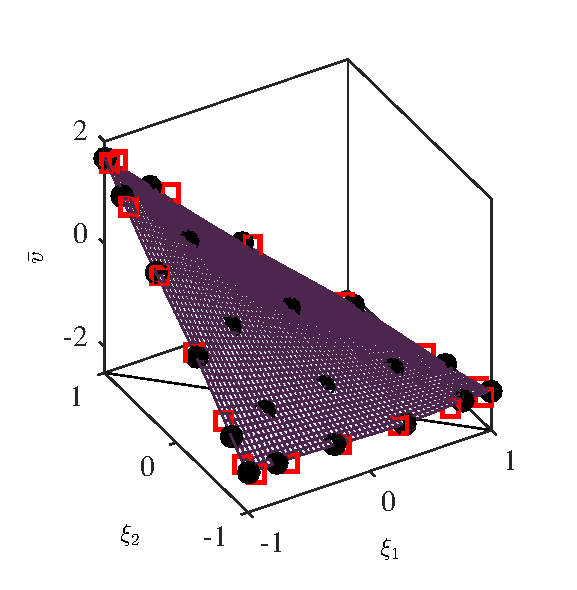
\includegraphics[width = 0.5\textwidth]{\lfsdir/figs/boundary_effect.eps}
\caption{Solution values after filtering with boundary component exclusively, $\vec{\bar{v}} = \mat{B}\vec{v^*}$, where  $\vec{v^*} = a\vec{\xi^*_1} + b\vec{\xi^*_2} + c$ for some constants $a,b,c$. Red squares show the values of the solution at the boundaries, filled black circles show the filtered values of the solution at the interior points, and the meshed surface shows the polynomial representation of the solution.} 
\label{fig:boundary_effect}
\end{figure}

Figure \ref{fig:boundary_effect_oscillatory} illustrates how the boundary filtering component would behave in the case the boundary values are not coplanar. It is interesting to note that close to the corner $(\xi_1,\xi_2) = (-1,1)$, two boundary points with different values are close to an internal point. The value  of the filtered solution close to those boundary points assumes a value that is close to the average of the two.

The polynomial interpolation of the filtered interior values shows that the closer an interior point is to a boundary point, the more it will be influenced by such boundary point. This causes the filtered values close to the boundaries to get closer to the boundary values. This suggests that the boundary filtering component does in fact help in bringing the solution closer to satisfying the boundary conditions while diminishing oscillations within the element.

\begin{figure}
\centering
\includegraphics[width = 0.5\textwidth]{\lfsdir/figs/boundary_effect_oscillatory.eps}
\caption{Solution values after filtering with boundary component exclusively, $\vec{\bar{v}} = \mat{B}\vec{v^*}$, where   ${v_i^*} = \sin{(k\xi^*_{i1})} + \cos{(k\xi^*_{i2})} $, $k=500$. Red squares show the values of the solution at the boundaries, filled black circles show the filtered values of the solution at the interior points, and the meshed surface shows the polynomial representation of the solution.} 
\label{fig:boundary_effect_oscillatory}
\end{figure}

\subsection{Filtered Solutions}
No filtering component is used solely by itself. The factor $\alpha$ in Equation \ref{eqn:filter_form} determines how much weight to give to each component. Figure \ref{fig:filtered_solutions} illustrates the effect of the boundary values on a fully filtered solution, when $\alpha = 0.8$.

The internal filtering component reduces oscillations, while the boundary filtering component brings the interior values closer to the boundary values. By placing the boundary values on different planes, this effect becomes more evident.

\begin{figure*}
\hspace{-1cm}
\subfloat[$\beta = -0.75$\label{fig:filt_neg}]{%
\includegraphics[width=0.5\textwidth]{\lfsdir/figs/filter_tilt_neg.eps}
}
\hfill
\subfloat[$\beta = 0.75$\label{fig:filt_pos}]{%
\centering
\includegraphics[width=0.5\textwidth]{\lfsdir/figs/filter_tilt_pos.eps}
}
\caption{Solution values after filtering with both internal and boundary components, $\vec{\bar{v}} = \alpha\mat{T}\vec{v} + (1-\alpha)\mat{B}\vec{v^*}$, where $\alpha = 0.8$, ${v_i} = \sin{(k\xi_{i1})} + \cos{(k\xi_{i2})} $, $k=500$, $\vec{v^*} = \beta (-\vec{\xi^*_1} + \vec{\xi^*_2})$. Hollow black circles show the unfiltered solution at the interior points, transparent colored surface is the polynomial representation of the unfiltered solution, filled black circles show the filtered values of the solution at the interior points, hollow red squares show the value of the solution at the boundary points, and the meshed surface shows the polynomial representation of the filtered solution.}
\label{fig:filtered_solutions}

\end{figure*}
\vspace{.20in}

\section{Results}
\label{sec:results}
To test the filters' ability to increase general robustness of a high-order solver, we have implemented their formulation in \gls{hf} for triangular elements and performed simulations where the solver would become unstable otherwise. In addition, we analyze the impact the filters have on a well-resolved 2-D simulation.

We wanted to test the increase of robustness in extreme cases of grid coarseness, high Reynolds number, very low \gls{ma}, and moderate \gls{ma}. It is important to keep in mind that in these cases we are not seeking very accurate results, but rather robustness under all conditions. In order to popularize high-order methods, we need to make them as robust as their low-order counterparts while retaining their benefit of higher accuracy with less computational and setup effort.

The goal is to have a cheap stabilization strategy that preserves boundary conditions for cases in which the mesh is not necessarily perfectly appropriate for resolving the flow physics over the entire domain. This scenario arises frequently in industrial applications, where the mesh would be properly refined at regions of interest and coarse in regions that the engineer/scientist has decided are not as important for the problem at hand.

All the simulations that follow were performed using \gls{hf}\cite{lopez2014verification}. 2-D \gls{ns} equations are being solved, with varying values of \gls{ma}, \gls{re}, time-step ($\Delta t$), and filtering frequency. The common parameters are:
\begin{enumerate}[1.]
\item Four-stage, five-step, low-storage Runge-Kutta time-stepping method (\gls{rk45}) \cite{carpenter1994fourth} was used in the \gls{gpu}s, and forward Euler was used when running a simulation in CPUs
\item Polynomial solution representation ($p$) of order $4$. Rusanov Flux as a Riemann solver, and a \gls{ldg}~\cite{cockburn1998local} viscous flux.
\item Filters with width $h = 10$ and weighting parameter $\alpha = 0.8$.
\item Starting from uniform flow
\item Characteristic boundary conditions at the inflow and outflow. No-slip, isothermal wall boundary conditions at the cylinder's surface.
\item All quantities non-dimensionalized with free-stream temperature and cylinder wall temperature of $300$, reference length of $1$.
\item Flow properties: $\gamma = 1.4$, Prandtl number $\mathrm{Pr} = 0.72$, gas constant $R = 286.9 \frac{J}{Kg K}$, viscosity determined by Sutherland's law with reference temperature of $291.15 K$ and reference viscosity of $\mu = 1.827\mathrm{e}-5$
\end{enumerate}

Results of interest are shown in Table \ref{table:results}. Accuracy of the results is not expected. Nevertheless, as a reference, for the flow around a cylinder at \gls{re}$= 1e6$, $\bar{C_D} \approx 0.6$ in~\cite{achenbach1968distribution}, $\bar{C_D} \approx 0.4$ in \cite{roshko1961experiments} and $\St \approx  0.4$ in \cite{roshko1961experiments}. It is important to note that at a high \gls{re}, flow over a cylinder can result in a range of $\bar{C_D}$ and $\St$ values, as the results become highly sensitive to surface roughness and the level of free-stream turbulence~\cite{zdravkovich1997flow}. The experimental values of $\bar{C_D}$ vary from 0.17 to 0.40, and those of $\St$ from 0.18 to 0.50.

Because of the results obtained in Case 4, it is good to keep in mind that for flow around a cylinder at \gls{re}$\approx 2e2$, $\bar{C_D} \approx 1.18$ in \cite{roshko1961experiments} and $\St \approx  0.2$ in \cite{roshko1961experiments}. 


\begin{table}
%\begin{adjustwidth}{-2.1cm}{}
%    \centering
    \cellspacebottomlimit=5pt
    \cellspacetoplimit=5pt
%      \begin{center}                % keep track of old \tabcolsep
        \setlength{\oldtabcolsep}{\tabcolsep}     % 6.0pt
        \setlength{\tabcolsep}{0pt}               % so coloring doesn't run off
                                                  % ends of the table
        \renewcommand{\arraystretch}{2}         % because math expressions
                                                  % almost run into each other

\def \spacing {0.4cm}
\hspace{-2.5cm}
\begin{tabular}{c <{\hspace{\len}}c <{\hspace{\spacing}} 
c <{\hspace{\spacing}}
c<{\hspace{\spacing}} c<{\hspace{\spacing}} c<{\hspace{\spacing}} c<{\hspace{\spacing}} c<{\hspace{\spacing}} c <{\hspace{\spacing}} c <{\hspace{\spacing}} c}
          \toprule
Case & $\Ma$  & $\Delta t$ & $n_F$ & $\bar{C_D}$  &  $\mathrm{St}$ & \specialcell[b]{Flow time \vspace{-0.2cm}\\(s)} & Time steps  & \specialcell[b]{Wall time \vspace{-0.2cm}\\(hours)}& \specialcell[b]{Computing \vspace{-0.2cm}\\ Resources}\\
          \specialrule{\lightrulewidth}{0pt}{0pt} % so row-coloring aligns

1 & $0.2$ &  $5e-5$ &$1000$ &$0.9256$ & $0.1600$ & $1.2069$ &$1,675,700$ & $12.65$&  1 4-core i7 CPU \\
2 & $0.077$ & $5e-5$ &$1000$ & $0.9314$ & $0.1627$ & $15.44$ & $8,252,500$ & $11.78$ & 1 \gls{gpu}\\
3 & $0.87$ & $5e-5$ &$100$ & $1.8383$ & $0^*$ & $1.3833$ & $8,355,256$ & $12.63$ & 1 \gls{gpu}\\
4 & $0.0077$ & $1.25e-5$ &$1000$ & $ 1.18$ & $0.20$ & $53.44$ & $11,428,000$ & $59.51$ & 2 \gls{gpu}s\\

          \bottomrule
        \end{tabular}

      \caption{Summary of simulation results. All cases were run at $\Re = 1e6$ with polynomial representation of order $4$. Cases 1-3 were run using the mesh shown in Figure \ref{fig:meshes}. Case 4 was run using the mesh shown in Figure \ref{fig:meshes2}. Cases with $0^*$ Strouhal number reached an artificial steady-state.}
      \label{table:results}
%      \end{adjustwidth}
    \end{table}


\subsection{Stabilization Strategy}
In the simulations presented here, the solution inside every element in the entire domain is being filtered using Equation \ref{eqn:filter_form} every $n_F$ time-steps, where $n_F$ is an integer to be determined. No sensor is being used to detect problems in the flow.

The frequency of filter application is being chosen in the following heuristic way:
\begin{enumerate}[1.]
\item \label{item:start}Start the simulation with a specific time step and no filtering. Record at what time-step the simulation ends prematurely (produces Nan values) and note the value of the residuals at the last valid time-step.  This step usually takes no more than 1 minute.
\item \label{item:halve_dt}To ensure the simulation is ending prematurely because of grid resolution problems or presence of sharp gradients, and not because of an unstable time step, halve the time step and run the simulation again.
\item \label{item:check_res} Wait for the simulation to exit prematurely. If the residual at this last exit is close in value to the previous exiting residual, the time step in Step \ref{item:halve_dt} was stable. Set the new time step to the time step in \ref{item:halve_dt}. Otherwise, record the exiting residual and go back to Step \ref{item:halve_dt}.
\item Now that a stable time step has been found, apply the filter to the simulation every $n_F$ time steps, where $n_F$ is about $90\%$ of the number of imte-steps it took the simulation to become unstable when unfiltered.
\end{enumerate}

It would certainly be desirable to filter the solution at elements where a problem is detected. Nevertheless, this heuristic approach has so far enabled the stabilization of every case tried and de-couples the effectiveness of the filters from possible shortcomings of aliasing/shock sensors.

\subsection{Coarse mesh used in simulations}
In these tests, we have used the very coarse triangular mesh with $714$ elements shown in Figure \ref{fig:meshes}. The boundary layer is purposefully not resolved properly, as we would like to induce aliasing errors in the unfiltered calculation.

\begin{figure*}
\hspace{-1cm}
\subfloat[Full mesh view \label{fig:mesh}]{%
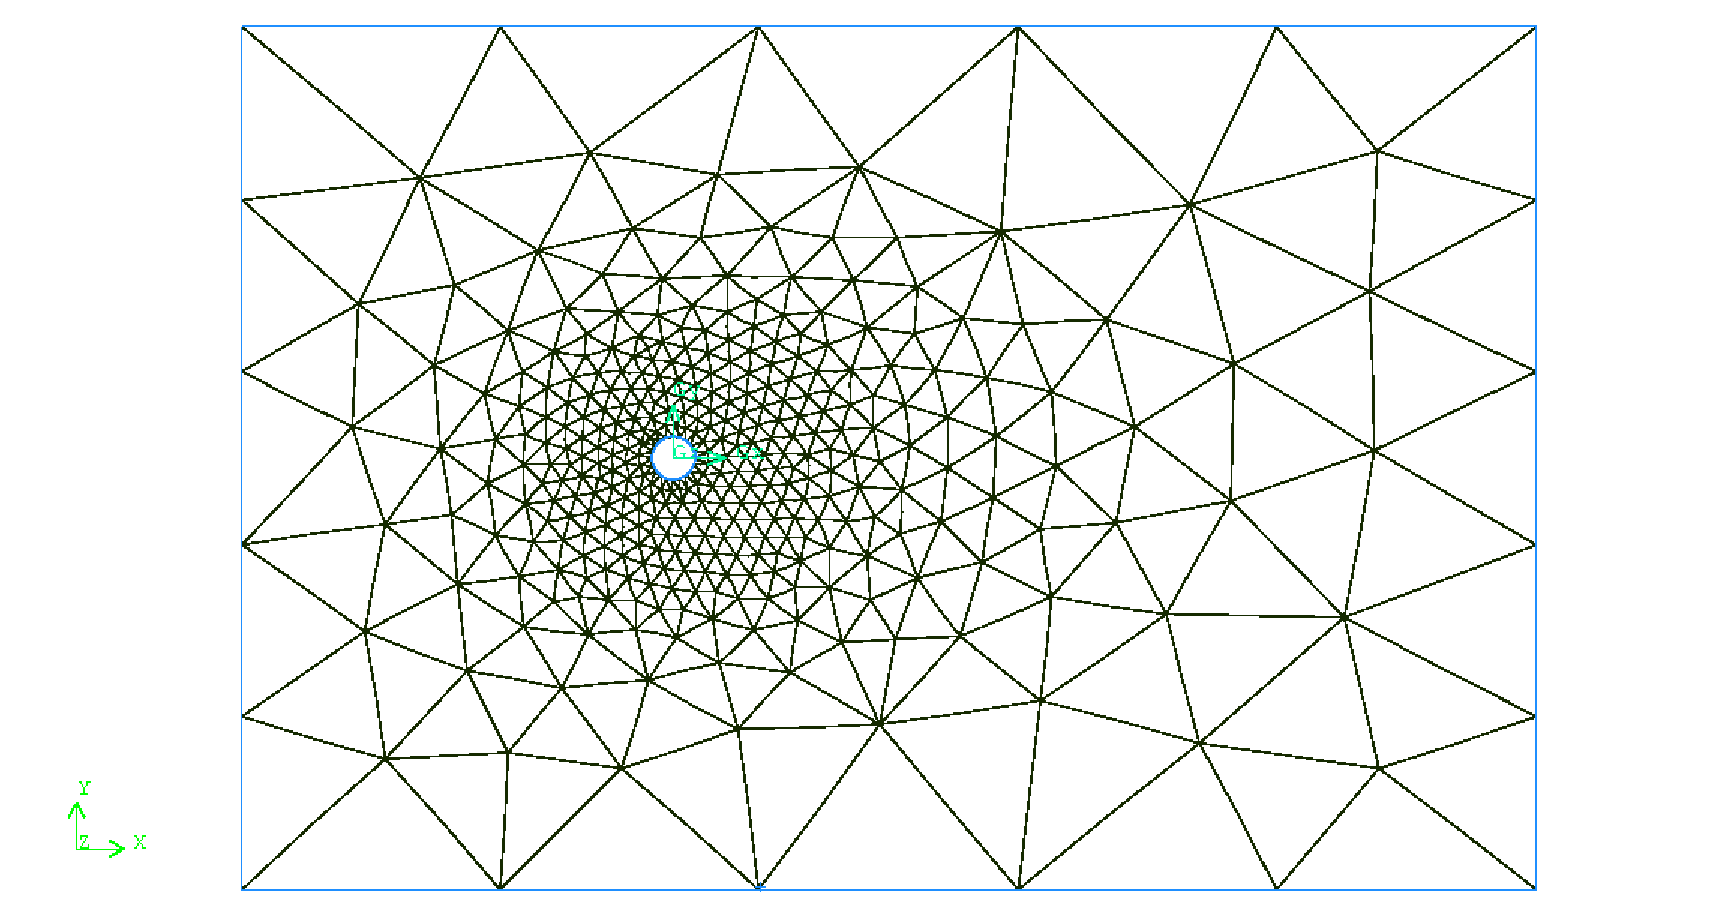
\includegraphics[width=0.55\textwidth]{\lfsdir/figs/MESH2.eps}
}
\hfill
\subfloat[Close-up view \label{fig:mesh_close}]{%
\centering
\includegraphics[width=0.55\textwidth]{\lfsdir/figs/MESH_CLOSE.png}
}
\caption{Unstructured, coarse mesh of a circular cylinder with $714$ triangular elements. Elements adjacent to the cylinder have quadratic edges.}
\label{fig:meshes}

\end{figure*}

\subsection{Flow Around a Circular Cylinder, $\bf Re =  10^6, Ma = 0.2$}
This was the first simulation performed after implementing the filters in \gls{hf}, so the \gls{gpu} implementation was not available then. The time-stepping scheme used here is simply forward Euler.

Figure \ref{fig:Ma0.2Re1e6_Ma} shows ``pretty pictures" resulting from the simulation. A video of this simulation is linked \href{https://youtu.be/b6kx8-jrK6Q}{here}.

It is interesting to note that there is a very dissipative form of vortex shedding occurring. The wake region is long, as in lower \gls{re}-number cases.

The simulation remained stable throughout and no human intervention was performed while it was occurring, from the start in uniform flow to the moment it was stopped.

From this experiment, it is unclear what portion of the numerical dissipation arises from the coarse discretization and what portion is due to the filtering operation.

This case demonstrates that the stabilization strategy can work well in cases where the mesh is improperly refined: they stabilize the solution and preserve the boundary conditions.

\begin{figure*}
\hspace{-1cm}
\subfloat[Full view \label{fig:Ma0_2Re1e6_Ma_far}]{%
\includegraphics[width=0.55\textwidth]{\lfsdir/figs/Ma0_2--Re1e6_Ma.png}
}
\hfill
\subfloat[Close-up view \label{fig:Ma0_2Re1e6_Ma_close}]{%
\centering
\includegraphics[width=0.55\textwidth]{\lfsdir/figs/Ma0_2--Re1e6_Ma_closeup.png}
}
\caption{Flow past a cylinder. $\Re = 1e6, \Ma = 0.2, p = 4$}
\label{fig:Ma0.2Re1e6_Ma}

\end{figure*}

\subsection{High Reynolds Number, Flow Around a Circular Cylinder, $\bf Re = 10^6, Ma = 0.077$}
This was the first simulation performed using \gls{gpu}s. The lower \gls{ma} case was of interest, as \gls{hf} had not been able to run full simulations of flows with \gls{ma}$< 0.2$.

Figure \ref{fig:Ma0.077Re1e6_Ma} shows the colorful results for this case. Once again, the boundary conditions are satisfied and the simulation is stabilized without further intervention. The same time-step size was used as in the previous case in order to leave as many parameters as possible unchanged.

A video of this simulation is linked \href{https://youtu.be/EymTVFzyPcA}{here} in real-time, and \href{https://youtu.be/8ZH349_GRUA}{here} at 0.1$\times$. A feature of these simulations that can only be appreciated by watching the linked videos is that the filters have a visible effect on the regions where aliasing and instabilities are expected: the rear part of the cylinder and the boundary layer. However, even though the filters are being applied everywhere, smooth, well-resolved regions of the flow look unchanged. To what extent the smooth regions remain unchanged has not been quantified.

\begin{figure*}
\hspace{-1cm}
\subfloat[Full view \label{fig:Ma0_077Re1e6_Ma_far}]{%
\includegraphics[width=0.55\textwidth]{\lfsdir/figs/Ma0_077--Re1e6_Ma.png}
}
\hfill
\subfloat[Close-up view \label{fig:Ma0_077Re1e6_Ma_close}]{%
\centering
\includegraphics[width=0.55\textwidth]{\lfsdir/figs/Ma0_077--Re1e6_Ma_closeup.png}
}
\caption{Flow past a cylinder. \gls{re}$= 1e6$, \gls{ma} $= 0.077, p = 4$}
\label{fig:Ma0.077Re1e6_Ma}

\end{figure*}

%\subsection{High Reynolds Number, Flow Around a Circular Cylinder, $\bf Re = 10^6, Ma = 0.85$}

\begin{figure*}
\hspace{-1cm}
\subfloat[Full view \label{fig:Ma0_87Re1e6_Ma_unstable_far}]{%
\includegraphics[width=0.55\textwidth]{figs/Ma0_87--Re1e6_Ma.png}
}
\hfill
\subfloat[Close-up view \label{fig:Ma0_87Re1e6_Ma__unstable_close}]{%
\centering
\includegraphics[width=0.55\textwidth]{figs/Ma0_87--Re1e6_Ma_closeup.png}
}

\hspace{-1cm}
\subfloat[Close-up view \label{fig:Ma0_87Re1e6_P__unstable}]{%
\centering
\includegraphics[width=0.55\textwidth]{figs/Ma0_87--Re1e6_P.png}
}
\hfill
\subfloat[Close-up view \label{fig:Ma0_87Re1e6_P__unstable_close}]{%
\centering
\includegraphics[width=0.55\textwidth]{figs/Ma0_87--Re1e6_P_closeup.png}
}
\caption{$\Re = 1e6, \Ma = 0.87, p = 4$}
\label{fig:Ma0.87Re1e6_unstable_Ma}
\end{figure*}

\subsection{High Reynolds Number, Flow Around a Circular Cylinder, $\bf Re = 10^6, Ma = 0.87$}

This case encompasses all potential sources of instabilities in a high-order solver: poor resolution, aliasing, and sharp gradients. Figure \ref{fig:Ma0.87Re1e6} shows plots of the solution. The simulation shows a clear un-physical asymmetry due to the coarseness of the mesh. Nevertheless, the no-slip boundary conditions are being satisfied and the shock is present. 

Because of the coarseness of the mesh and the high-gradients present in the solution, quite a lot of filtering had to occur. This forced the flow to a ``steady state" and shown in the Residual and $C_D$ plots in Figure \ref{fig:Ma0.87Re1e6_history}.

\begin{figure*}
\hspace{-1cm}
\subfloat[Full view \label{fig:Ma0_87Re1e6_Ma_far}]{%
\includegraphics[width=0.55\textwidth]{\lfsdir/figs/Ma0_87--Re1e6_Ma_stable.png}
}
\hfill
\subfloat[Close-up view \label{fig:Ma0_87Re1e6_Ma_close}]{%
\centering
\includegraphics[width=0.55\textwidth]{\lfsdir/figs/Ma0_87--Re1e6_Ma_stable_closeup.png}
}

\hspace{-1cm}
\subfloat[Full view \label{fig:Ma0_87Re1e6_P_stable}]{%
\centering
\includegraphics[width=0.55\textwidth]{\lfsdir/figs/Ma0_87--Re1e6_P_stable.png}
}
\hfill
\subfloat[Close-up view \label{fig:Ma0_87Re1e6_P_stable_close}]{%
\centering
\includegraphics[width=0.55\textwidth]{\lfsdir/figs/Ma0_87--Re1e6_P_stable_closeup.png}
}
\caption{Flow past a cylinder. \gls{re}$= 1e6$, \gls{ma} $= 0.87, p = 4$}
\label{fig:Ma0.87Re1e6}

\end{figure*}

Values of $C_D$ and residual history are shown in Figure \ref{fig:Ma0.87Re1e6_history}. The value of drag ``converges" after time-step $1.846e6$. The residual in the energy conservation equation also ``converges" to a zig-zag pattern after this iteration. Figure \ref{fig:rhoE_res_history} shows the energy residual in the last few thousand time-steps. The sharp decrease in residual magnitude reveals the time-steps at which the filter is being applied.

\begin{figure*}
\subfloat[Drag coefficient history over entire simulation run. ``Steady state" is reached at time-step $1.846e6$. \label{fig:cd_history}]{%
\includegraphics[width=0.55\textwidth]{\lfsdir/figs/unstable_c_d.eps}
}
\hfill
\subfloat[Energy residual history over the last few thousand time-steps \label{fig:rhoE_res_history}]{%
\centering
\includegraphics[width=0.55\textwidth]{\lfsdir/figs/unstable_rhoE_res.eps}
}
\caption{History of $C_D$ and energy residual of simulation in Figure \ref{fig:Ma0.87Re1e6}}
\label{fig:Ma0.87Re1e6_history}

\end{figure*}

\subsection{High Reynolds Number, Flow Around a Circular Cylinder, $\bf Re = 10^6, Ma = 0.0077$, less-coarse mesh}
This case was run with the more refined mesh seen in Figure \ref{fig:meshes2}. This mesh is still coarse for standard turbulent computations. It is interesting to note that the predicted $C_D = 1.18$ and $\mathrm{St} = 0.20$ match experimental results for \gls{re}$= 2e2$. This phenomenon could imply that the grid of the stabilized simulation determines the effective Reynolds number being simulated.

A real-time video of this simulation is linked \href{https://youtu.be/XSzWPn2fZ90}{here} for Mach contours, and \href{https://youtu.be/_zIbZgHjepY}{here} for vorticity strength contours. The filters stabilized this almost-incompressible simulation without a problem.


\begin{figure*}
\hspace{-1cm}
\subfloat[Full mesh view \label{fig:mesh2}]{%
\includegraphics[width=0.55\textwidth]{\lfsdir/figs/cylinder_fine_v2.png}
}
\hfill
\subfloat[Close-up view \label{fig:mesh2_close}]{%
\centering
\includegraphics[width=0.55\textwidth]{\lfsdir/figs/mesh_closeup_2.png}
}
\caption{Unstructured, coarse mesh of a circular cylinder with 5,616 triangular elements. Elements adjacent to the cylinder have quadratic edges.}
\label{fig:meshes2}

\end{figure*}


\begin{figure*}
\hspace{-1cm}
\subfloat[Full view \label{fig:Ma0_0077Re1e6_Ma_far}]{%
\includegraphics[width=0.55\textwidth]{\lfsdir/figs/Ma0_0077--Re1e6_Ma.png}
}
\hfill
\subfloat[Close-up view \label{fig:Ma0_0077Re1e6_Ma_close}]{%
\centering
\includegraphics[width=0.55\textwidth]{\lfsdir/figs/Ma0_0077--Re1e6_Ma_closeup.png}
}
\caption{Flow past a cylinder. \gls{re}$= 1e6$, \gls{ma} $= 0.0077, p = 4$}
\label{fig:Ma0.0077Re1e6_Ma}

\end{figure*}

% !TEX root = ./thesis.tex
\subsection{Effects of Filtering in a Well-resolved Simulation}
\label{sec:filteringEffects}

This Section shows that the use of \gls{lfs} has effects similar to using artificial viscosity. The previous results show that \gls{lfs} filters can stabilize even the most extreme of circumstances. What about the effect of using \gls{lfs} filters in more reasonable conditions?

The case of 2-D flow over a circular cylinder at \gls{re} $=3,900$, \gls{ma} $=0.1$ has been selected given the good amount of computational results for it. The thesis by Beaudan \cite{beaudan1994numerical} provides a very thorough discussion of the physics of the 3-D problem and results of simulations with structured high-order methods.

At \gls{re} $=3,900$, a proper simulation of flow around a circular cylinder must be 3-D \cite{breuer1998large}. In fact, previous 2-D simulations of this case have shown the flow to be highly asymmetric \cite{breuer1998large}. The aim of the simulations presented here is not to predict experimental results, but rather to provide an understanding of how the flow will be affected by the use of \gls{lfs} filters. We will see that the \gls{lfs} filters act as artificial viscosity: flow that would otherwise exhibit chaotic behavior becomes periodic. A similar transition from chaotic to periodic behavior due to added dissipation (via turbulence modeling) has been observed in \gls{urans} simulations \cite{catalano2003numerical}.

\subsubsection{Setup}
\label{sec:filterEffectsSetup}

We first generate a grid for a $2^{\mathrm{nd}}$ order method that resolves the $y+$ scales around the cylinder. We then generate grids that maintain close to the same number of \gls{dof} for a \nth{5}  and \nth{6} spatial order of accuracy scheme. We perform the simulation of \gls{re}$=3.9e3$ past a circular cylinder using the \nth{5} and \nth{6} order schemes in the different grids. The aims of this setup are to:
\begin{enumerate}
\item Have a well-resolved, baseline case
\item Visualize the effects of changing the spatial order of accuracy while maintaining the number of \gls{dof} almost constant
\item Visualize the effects of using an under-resolved grid
\item Visualize the effects of using \gls{lfs} filters in different grids with different spatial orders of accuracy
\end{enumerate}

A baseline case with a \nth{6} order accurate in space scheme was attempted while maintaining the same number of degrees of freedom as the case with the $2^{\mathrm{nd}}$ order scheme. However, the non-linearities within the relatively large elements elements prevented the simulation from completing without intervention. However, a simulation with filtering in the same grid with the same order of accuracy did run to completion.

In addition, to compare the effects of filtering versus running a slightly unresolved simulation, an unfiltered case of a slightly unresolved grid was run with a \nth{5} order scheme.

Finally, a well resolved, yet filtered, simulation with the \nth{5} order scheme was performed.

All cases ran with the same non-dimensional time-step of $\Delta t = 1e-5$ for a non-dimensional time of $t = 64.7$. Given that \gls{ma} $=0.1$, temperature of air simulated was $300K$, $\gamma = 1.4$, and the reference length was $1$ meter, the physical time-step was $2.88e-6$ seconds and the physical simulation time was $1.86$ seconds.

Filtering is performed with a value of $h = 10$ in Equation \eqref{eq:sharp_spectral} and $\alpha = 0.8$ in Equation \eqref{eqn:filter_form}. All conservation fields are filtered every 500 time-steps, so every $5e-2$ non-dimensional time units, or every $1.44e-3$ seconds. The filtering procedure was kept the same to isolate the effects of filtering. In practice, a sensor should be used in order to only filter the elements where instabilities could arise.


\subsubsection{Results and Discussion}
\label{sec:filterEffectsResults}

Table \ref{table:filteringEffect_simSummary} summarizes all the cases run and provides hyperlinks to videos of the resulting flow simulations. The value of \gls{st} provided reflects the peak \gls{st} of the lift coefficient power spectrum.

All cases display the following phases: a pair of vortices strengthen behind the cylinder, the vortices elongate and the drag coefficient decreases, asymmetries in the solution trigger vortex shedding, the vortex growth and shedding process transitions into a quasiperiodic (when not filtered) or periodic (when filtered) behavior.

\begin{table}
%\begin{adjustwidth}{-2.1cm}{}
%    \centering
\cellspacebottomlimit=5pt
\cellspacetoplimit=5pt
%      \begin{center}                % keep track of old \tabcolsep
\setlength{\oldtabcolsep}{\tabcolsep}     % 6.0pt
\setlength{\tabcolsep}{0pt}               % so coloring doesn't run off
% ends of the table
\renewcommand{\arraystretch}{2}         % because math expressions
% almost run into each other

\def \spacing {0.4cm}
\hspace{-0.5cm}
\begin{tabular}{c <{\hspace{\len}} c <{\hspace{\len}} c <{\hspace{\len}} c <{\hspace{\spacing}} 
c <{\hspace{\spacing}}
c<{\hspace{\spacing}} c<{\hspace{\spacing}} c<{\hspace{\spacing}} c}
\toprule
Case & $P$  & Mesh & Filtered & Grid & $\#$ \gls{dof} & \specialcell[b]{$C_L$ and $C_D$ vs. $t$ \vspace{-0.2cm}\\Figure}   &  \specialcell[b]{\gls{st}} & \specialcell[b]{Video} \\
\specialrule{\lightrulewidth}{0pt}{0pt} % so row-coloring aligns

\hypertarget{caseA}{A} & 1 &  \ref{fig:mesh_case_A} & No & \ref{fig:mesh_case_A} & 1,579,620 & \ref{fig:history_P1_noFilt_mesh1} & 0.19 & \href{https://www.youtube.com/watch?v=mtUrv-Aj_y0}{link} \\
\hypertarget{caseB}{B} & 4 & \ref{fig:mesh_case_BDG} & No & \ref{fig:mesh_case_BDG} & 1,398,780 & \ref{fig:history_P4_noFilt_mesh4} & 0.17 & \href{https://www.youtube.com/watch?v=FpyAf08kz7A}{link} \\
\hypertarget{caseC}{C} & 4 & \ref{fig:mesh_case_C} & No & \ref{fig:mesh_case_C} & 703,260 & \ref{fig:history_P4_noFilt_mesh6} & 0.17 & \href{https://www.youtube.com/watch?v=Tud7N1tmmrA}{link} \\
\hypertarget{caseD}{D} & 4 & \ref{fig:mesh_case_BDG} & Yes & \ref{fig:mesh_case_BDG} & 1,398,780 & \ref{fig:history_P4_filt_mesh4} & 0.25 & \href{https://youtu.be/H1xKenZ2g6Q}{link} \\
\hypertarget{caseE}{E} & 5 & \ref{fig:mesh_case_EF} & No & \ref{fig:mesh_case_EF} & 1,362,396 & Unstable & N/A & N/A \\
\hypertarget{caseF}{F} & 5 & \ref{fig:mesh_case_EF} & Yes & \ref{fig:mesh_case_EF} & 1,362,396 & \ref{fig:history_P5_filt_mesh5} & 0.21 & \href{https://www.youtube.com/watch?v=FMZBi285alk}{link} \\
\hypertarget{caseG}{G} & 5 & \ref{fig:mesh_case_BDG} & Yes & \ref{fig:mesh_case_BDG} & 1,958,292 & \ref{fig:history_P5_filt_mesh4} & 0.25 & \href{https://www.youtube.com/watch?v=cmIKRwJXoME}{link} \\

\bottomrule
\end{tabular}
\caption{Simulation results that illustrate effect of filtering, changing meshes, and varying the spatial order of accuracy. All cases were run at \gls{ma} $=0.1$, \gls{re}$ = 3.9e3$.}
\label{table:filteringEffect_simSummary}
\end{table}


\begin{figure}
\centering
\includegraphics[width = 1\textwidth]{\lfsdir/figs/mesh_images/cylinder_1stOrder_Re3-6e3_fine1_mod.png}
\caption{Mesh used in case A in Table \ref{table:filteringEffect_simSummary}. Contains 131,635 triangular elements with second order edges.} 
\label{fig:mesh_case_A}
\end{figure}

\begin{figure}
\centering
\includegraphics[width = 1\textwidth]{\lfsdir/figs/mesh_images/cylinder_4thOrder_Re3-9e3_mod.png}
\caption{Mesh used in cases B, D, and G in Table \ref{table:filteringEffect_simSummary}. Contains 23,313 triangular elements with second order edges.} 
\label{fig:mesh_case_BDG}
\end{figure}

\begin{figure}
\centering
\includegraphics[width = 1\textwidth]{\lfsdir/figs/mesh_images/cylinder_6thOrder_Re3-9e3_mod.png}
\caption{Mesh used in case C in Table \ref{table:filteringEffect_simSummary}. Contains 11,721 triangular elements with second order edges.} 
\label{fig:mesh_case_C}
\end{figure}

\begin{figure}
\centering
\includegraphics[width = 1\textwidth]{\lfsdir/figs/mesh_images/cylinder_5thOrder_Re3-9e3_mod.png}
\caption{Mesh used in cases E and F in Table \ref{table:filteringEffect_simSummary}. Contains 16,219 triangular elements with second order edges.}
\label{fig:mesh_case_EF}
\end{figure}

% % % % % % % % % % % % % % % % % % % % % % % %  Simulation Results

\begin{figure}
\centering
\includegraphics[width = 1\textwidth]{\lfsdir/figs/history_P1_noFilt_mesh1.png}
\caption{Case A in Table \ref{table:filteringEffect_simSummary} lift coefficient, \gls{st} power spectrum, and drag coefficient. Case is not filtered and uses mesh \ref{fig:mesh_case_A} with $P=1$. }  
\label{fig:history_P1_noFilt_mesh1}
\end{figure}

\begin{figure}
\centering
\includegraphics[width = 1\textwidth]{\lfsdir/figs/history_P4_noFilt_mesh4.png}
\caption{Case B in Table \ref{table:filteringEffect_simSummary} lift coefficient, \gls{st} power spectrum, and drag coefficient. Case is not filtered and uses mesh \ref{fig:mesh_case_BDG} with $P=4$.} 
\label{fig:history_P4_noFilt_mesh4}
\end{figure}

\begin{figure}
\centering
\includegraphics[width = 1\textwidth]{\lfsdir/figs/history_P4_noFilt_mesh6.png}
\caption{Case C in Table \ref{table:filteringEffect_simSummary} lift coefficient, \gls{st} power spectrum, and drag coefficient. Case is not filtered and uses mesh \ref{fig:mesh_case_C} with $P=4$.} 
\label{fig:history_P4_noFilt_mesh6}
\end{figure}

\begin{figure}
\centering
\includegraphics[width = 1\textwidth]{\lfsdir/figs/history_P4_filt_mesh4.png}
\caption{Case D in Table \ref{table:filteringEffect_simSummary} lift coefficient, \gls{st} power spectrum, and drag coefficient. Case is filtered and uses mesh \ref{fig:mesh_case_BDG} with $P=4$.} 
\label{fig:history_P4_filt_mesh4}
\end{figure}

\begin{figure}
\centering
\includegraphics[width = 1\textwidth]{\lfsdir/figs/history_P5_filt_mesh5.png}
\caption{Case F in Table \ref{table:filteringEffect_simSummary} lift coefficient, \gls{st} power spectrum, and drag coefficient. Case is filtered and uses mesh \ref{fig:mesh_case_EF} with $P=5$.} 
\label{fig:history_P5_filt_mesh5}
\end{figure}

\begin{figure}
\centering
\includegraphics[width = 1\textwidth]{\lfsdir/figs/history_P5_filt_mesh4.png}
\caption{Case G in Table \ref{table:filteringEffect_simSummary} lift coefficient, \gls{st} power spectrum, and drag coefficient. Case is filtered and uses mesh \ref{fig:mesh_case_BDG} with $P=5$.} 
\label{fig:history_P5_filt_mesh4}
\end{figure}

\emph{Effect of changing the spatial order of accuracy while keeping the number of \gls{dof} constant.} Cases \hyperlink{caseA}{A} ($P=1$) and \hyperlink{caseB}{B} ($P=4$) keep close to the same number of \gls{dof}. Their lift coefficient power spectra show that the main vortex shedding frequencies are similar. Their drag coefficient figures reveal that \hyperlink{caseB}{Case B}, as expected, experiences less numerical dissipation; the initial vortices detach later than in \hyperlink{caseA}{Case A}. In addition, the drag coefficient plot in \hyperlink{caseB}{Case B} shows the presence of fairly small structures. \hyperlink{caseA}{Case A} seems to diffuse such structures. This effect can be seen in the corresponding videos as well.

\emph{Effect of changing the number of \gls{dof} while maintaining the spatial order of accuracy constant.} Cases \hyperlink{caseB}{B} and \hyperlink{caseC}{C} differ only in the mesh, \hyperlink{caseC}{Case C} has about half as many \gls{dof} as \hyperlink{caseB}{B}. Both cases have a peak in the lift coefficient power spectrum at \gls{st}$=0.17$. As can be seen in the videos and the drag coefficient plots, smaller structures are present in \hyperlink{caseB}{Case B}, however, \hyperlink{caseC}{Case C} still captures smaller structures than \hyperlink{caseA}{A} ($P=1$) while using half as many \gls{dof} and introduces less dissipation as demonstrated by \hyperlink{caseC}{Case C}'s delayed start of vortex shedding. The strength of the peak at \gls{st}$=0.17$ has decreased in \hyperlink{caseC}{Case C}. This points to the fact that higher dissipation increases the strength of shearing forces on the vortices, thus prompting earlier detachment and smaller lift coefficient oscillation amplitude.

\emph{Effect of using \gls{lfs} filters.}  Cases \hyperlink{caseB}{B} and \hyperlink{caseD}{D} differ only in the filtering. \hyperlink{caseD}{Case D} is filtered. The most salient effect of filtering is that the filtered solution starts shedding vortices earlier, sheds vortices periodically (as opposed to quasiperiodically), and very fine structures are almost non-existent. Indeed the flow looks like the case of \gls{re}$=100$ in Figure \ref{cylinder_3}, yet it predicts a higher mean drag coefficient. The power spectrum of the lift coefficient has very little energy at high values of \gls{st}. This is consistent with the desire of filtering specific frequencies from the simulation. Unfortunately the author could not find studies performed regarding the effect of artificial viscosity on the properties of chaotic flows. Nevertheless, the behavior observed in the filtered solution is consistent with what would be expected of a more viscous flow.

\emph{Effect of spatial order of accuracy on filtered simulations.} Cases \hyperlink{caseD}{D} and \hyperlink{caseG}{G} are both filtered and differ only in the spatial order of accuracy. The two simulations are nearly identical. This result is very encouraging: the filtering formulation maintains the spectral properties independent of the spatial order of accuracy. Recall that the filtering matrices are different for the different schemes. This means that the \gls{lfs} filters' spectral properties can be relied on when developing or using \gls{sgs} models.

\emph{Effect of the mesh on filtered simulations.} Cases \hyperlink{caseF}{F} and \hyperlink{caseG}{G} are both filtered and differ only in the mesh used. The peak \gls{st} number for the coarser grid, \hyperlink{caseF}{Case F}, is lower and its predicted average drag coefficient is lower. This result reflects the general high dependence of simulation results on the grid quality. The grid used in \hyperlink{caseF}{Case F} could not produce a stable unfiltered simulation result even with smaller time-steps. It is possible the shift in the drag coefficient is a reflection of the mesh's improper resolution. This shows that the \gls{lfs} filters could in some cases provide stability at the expense of accurate physics and confirms that \gls{lfs} filters de-couple stability from proper resolution.



% % % % % % % % % % % % % % % % % % % %  Conclusion
\subsubsection{Conclusion}
\label{sec:filterEffectsConclusion}
In the simulations summarized in Table \ref{table:filteringEffect_simSummary}, it was possible to isolate the effects of filtering on a \gls{re}$=3.9e3$, \gls{ma}$=0.1$ 2-D flow past a circular cylinder. The unfiltered solutions in different grids obtained with different spatial orders of accuracy displayed minor differences: all unfiltered flows showed quasiperiodic flow with a peak lift coefficient power at a frequency of \gls{st}$\approx 0.18$. All filtered solutions exhibited an apparent regime change: the flow became periodic and the peak lift coefficient power occurred at a higher frequency.

It could be surmised that the \gls{lfs} filters showed the following strengths:
\begin{enumerate}
\item The scales filtered by \gls{lfs} filters are relative to the element size and virtually independent of the order of the basis polynomials, this could be leveraged in the development of \gls{sgs} models. This was demonstrated by the extremely similar results of Cases \hyperlink{caseD}{D} and \hyperlink{caseG}{G}, which were performed in the same grid with different orders of accuracy.
\item \gls{lfs} filters de-couple stability from proper simulation resolution. This could be very helpful when performing \gls{les} of turbulent flows. If proper resolution were required for stability, such cases would need to have a resolution close to that of \gls{dns}.
\end{enumerate}

The following was identified as a potential drawback:
\begin{enumerate}
\item Application of \gls{lfs} filters in the entirety of the simulation can cause an artificial regime change consistent with what would be expected of increasing viscosity in the flow. This calls for a selective application of \gls{lfs} filters.
\item Because the spectral properties of \gls{lfs} filters scale with the element size, results of flows filtered throughout are grid dependent. Once again, the use of sensors could ameliorate this grid dependence.
\end{enumerate}





\vspace{.20in}

\section{Conclusion}
\label{sec:conclusion}

We have suggested a formulation of \gls{lfs} filters for the stabilization of \gls{ns} solvers for unstructured grids that use a Finite Element Method-based approach to achieve high order spatial discretizations. This includes \gls{dg}, \gls{sd}, Spectral Element, and \gls{fr} methods. The filtering operation can be performed at individual elements and maintains a local stencil by using the element's solution and boundary values. This makes their implementation highly parallelizable.

The filters have been developed with the desired properties shown in Section \ref{sec:lfs_properties}. In essence, the filters have a spectral interpretation and satisfy boundary conditions asymptotically. The computational cost of applying a filtering operation to a single element is two small matrix multiplications. This low cost plus the compact stencil makes the \gls{lfs} filters a good alternative to using artificial dissipation. The main advantage of \gls{lfs} filters over artificial dissipation is that no modification needs to be made to the partial differential equations being solved.

We have shown by implementing the \gls{lfs} filters in \gls{hf} that little to no tuning is necessary to achieve stability in cases where instability is expected: coarse grids, high-\gls{re} flows, high-\gls{ma} flows, and low-\gls{ma} flows. In all cases, the filters preserved the boundary conditions, did not introduce visible flow anomalies, and allowed the flow to develop its natural features. The summary of results can be seen in Table \ref{table:results}.

Because the filter has a physical interpretation, \gls{sgs} modeling could be done with the classical physical arguments. A similar type of filter has been used by Lodato\cite{lodato2014structural} in the \gls{sd} scheme to do \gls{sgs} modeling rather than to stabilize the solution.

The unexpected finding that the filters could bring simulations in very coarse meshes to a pseudo-steady state opens up the possibility of using the \gls{lfs} filters as part of a pre-conditioning strategy or to start flow simulations from conditions more developed than uniform flow.

All algorithms are publicly available in the \gls{hf} \href{https://github.com/HiFiLES/HiFiLES-solver}{repository} under the branch ``\gls{lfs}-filters". The filters have been fully implemented for \gls{gpu}/CPU computations for triangular grids only.

%The results seen in \cite{asthana2014} are very promising, given that a double shock 2D simulation with $9^\text{th}$ order of accuracy are possible. We have recently submitted an article\cite{asthana2014} to JCP showing the promising results. Due to time constraints (the article was submitted on November 12, 2014), we have not produced results different to those in the article, but expect to have excellent results in the final version.
%
\vspace{.10in}

\section{Future Work}
\label{sec:future_work}
Implementation in 3D elements is straightforward and shall be the immediate course of action. 3D high-\gls{re} simulations had not been possible in \gls{hf} and it is expected stabilization with \gls{lfs} filters will enable them.

So far in all simulations the filters are acting on all elements in the domain with a pre-determined frequency. A more surgical approach to filtering is needed. As shown by Lv et al.~\cite{lv2015entropy}, localized and selective direct solution manipulation (limiting by multiplying the solution by a scalar while preserving the average within an element) can preserve the overall order of accuracy. The implementation of an aliasing/shock sensor is in order. Because the filters appear to have little effect on regions where the solution is well resolved, it is acceptable if the sensor is too conservative. The sensor proposed by Persson et al.~\cite{persson2006sub} for general elements and by Sheshadri et al.~\cite{Sheshadri2014} for tensor-product elements are prime candidates.

The filters are modifying all conservation variables within an element, and very likely key flow quantities like entropy and pressure are being disturbed. This disturbance needs to be quantified.

To prove the usefulness of the \gls{lfs} filters in a challenging simulation environment, it will be essential to assess their performance in a grid refined properly for the case at hand.
\vspace{-.20in}
